\chapter{Studi Literatur}

Pada bab ini, akan diisi oleh studi literatur, 
hal-hal yang berkaitan dengan topik persoalan tugas akhir 
akan dipaparkan dalam bab ini guna untuk memberikan informasi 
mengenai dasar teori dan studi yang dipakai. 
Bab ini diharapkan membantu pembaca untuk mengerti 
dalam membaca penelitian tugas akhir ini.

\section{\textit{Natural Language Processing}}

Pemrosesan Bahasa Alami (PBA) atau dalam bahasa Inggris dikenal dengan \textit{Natural Language Processing} (NLP) merupakan cabang dari ilmu komputer, kecerdasan buatan, dan linguistik yang berfokus pada interaksi antara komputer dan bahasa manusia. NLP bertujuan untuk memungkinkan komputer tidak hanya memahami dan menafsirkan bahasa manusia, tetapi juga untuk menghasilkannya dengan cara yang bermakna dan efektif. Hal ini dijelaskan oleh \citeauthor{nlp} \parencite{nlp}, menyatakan pentingnya NLP dalam membangun jembatan komunikasi antara manusia dan mesin.

Dalam beberapa dekade terakhir, NLP telah mengalami kemajuan yang signifikan, memungkinkan komputer tidak hanya memahami bahasa manusia tetapi juga merespons dengan cara yang semakin kompleks dan kontekstual. Teknologi seperti mesin penerjemah, asisten virtual, dan sistem rekomendasi semuanya memanfaatkan prinsip-prinsip NLP untuk berfungsi.

Salah satu tantangan utama dalam NLP adalah keragaman dan kompleksitas bahasa manusia. Bahasa penuh dengan nuansa, ambiguitas, dan struktur yang dapat bervariasi tergantung pada konteks dan budaya. Untuk mengatasi tantangan ini, berbagai tugas NLP telah didefinisikan dan dikembangkan untuk memecah masalah pemahaman bahasa menjadi komponen yang lebih kecil dan lebih spesifik.

Beberapa tugas NLP yang umum antara lain \textit{Part of Speech} (POS) \textit{Tagging}, \textit{Named Entity Recognition} (NER), \textit{Dependency Parsing}, \textit{Sentiment Analysis}, dan \textit{Summarization}. Masing-masing tugas ini menargetkan aspek tertentu dari pemahaman bahasa dan memiliki aplikasi praktisnya sendiri dalam berbagai bidang, mulai dari analisis teks hingga pengembangan sistem percakapan otomatis.
\subsection{\textit{Part of Speech} (POS) \textit{Tagging}}

\textit{Part of Speech (POS) Tagging}, adalah proses mengkategorikan setiap kata dalam teks ke dalam kelas kata tertentu berdasarkan definisi dan konteksnya. Misalnya, kata "berlari" mungkin diberi tag sebagai verba, sementara "cepat" sebagai adjektiva. Tujuan dari POS tagging adalah untuk memahami fungsi kata dalam kalimat, yang penting dalam banyak aplikasi NLP lainnya.
\subsection{\textit{Named Entity Recognition} (NER)}

\textit{Named Entity Recognition} (NER) adalah tugas mengidentifikasi dan mengklasifikasikan nama entitas dalam teks ke dalam kategori seperti nama orang, organisasi, lokasi, dan lainnya. Misalnya, dalam kalimat "Barack Obama lahir di Hawaii", "Barack Obama"  dikenali sebagai nama orang dan "Hawaii" sebagai lokasi.

\subsection{\textit{Dependency Parsing}}

\textit{Dependency Parsing} adalah proses menentukan hubungan gramatikal antara kata-kata dalam kalimat. Ini menghasilkan struktur pohon di mana simpul adalah kata-kata dan tepi menunjukkan hubungan ketergantungan antara kata-kata tersebut. Misalnya, dalam kalimat "Ani memberi buku kepada Budi", kata "memberi" mungkin memiliki hubungan dengan "Ani" sebagai subjek dan "buku" sebagai objek langsung.
\subsection{\textit{Sentiment Analysis}}

\textit{Sentiment Analysis} adalah tugas mengidentifikasi dan mengekstrak opini atau perasaan dari teks. Tujuannya adalah untuk menentukan apakah pendapat yang dinyatakan dalam teks adalah positif, negatif, atau netral. Misalnya, "Saya suka film ini" memiliki sentimen positif, sementara "Saya membenci makanan di restoran itu" memiliki sentimen negatif.
\subsection{\textit{Summarization}}

\textit{Summarization} adalah proses mengurangi teks panjang menjadi versi yang lebih pendek yang tetap mempertahankan informasi penting. Ada dua pendekatan utama dalam ringkasan: ekstraktif, di mana kalimat atau frasa diambil langsung dari teks asli, dan abstraktif, di mana informasi diringkas dengan kata-kata baru. Misalnya, artikel berita panjang tentang kejadian tertentu dapat diringkas menjadi beberapa kalimat yang mencakup poin utama.

\section{\textit{Transformer}}

\textit{Transformer} telah mengubah lanskap pemrosesan bahasa alami (NLP) dengan cara yang signifikan. Dalam makalah mereka, penulis memperkenalkan konsep baru yang disebut mekanisme self-attention \parencite{transformers}. Mekanisme ini memungkinkan setiap kata dalam input untuk memfokuskan pada kata-kata lain dalam sekuens yang sama, memberikan model kemampuan untuk memahami konteks dengan lebih baik. Ini berbeda dari pendekatan sebelumnya yang biasanya mengandalkan informasi lokal atau posisi tetap dalam sekuens.

Salah satu keunggulan utama dari mekanisme self-attention adalah kemampuannya untuk menangani sekuens dengan panjang yang berbeda dan memahami hubungan antar kata tanpa mempertimbangkan jarak antara mereka. Ini memungkinkan Transformer untuk memahami ketergantungan jarak jauh dalam teks, sesuatu yang sulit dicapai oleh arsitektur sebelumnya seperti RNN dan LSTM.

Selain itu, Transformer dirancang untuk paralelisasi, yang memungkinkannya dilatih dengan cepat pada perangkat keras modern. Ini mempercepat penelitian dan pengembangan dalam NLP dan memungkinkan pelatihan model skala besar seperti BERT dan GPT yang sekarang mendominasi bidang ini.

Sejak diperkenalkannya Transformer, banyak variasi dan peningkatan telah dikembangkan. Namun, prinsip dasar self-attention dan paralelisasi yang diperkenalkan oleh Transformer tetap menjadi inti dari banyak inovasi dalam NLP kontemporer.

\section{\textit{Bidirectional Encoder Representations from Transformers} \\ (BERT)}

BERT, yang merupakan singkatan dari \textit{Bidirectional Encoder Representations} from Transformers, adalah model pemrosesan bahasa alami yang diperkenalkan oleh Google pada tahun 2018 \parencite{bert}. BERT memanfaatkan arsitektur Transformer, yang telah kita bahas sebelumnya, untuk memahami konteks kata dalam teks dengan cara yang lebih mendalam daripada pendekatan sebelumnya.

Salah satu keunggulan utama BERT adalah pendekatannya yang \textit{bidirectional}. Sebagai gantinya dari hanya memahami teks dari kiri ke kanan atau sebaliknya, BERT memahami konteks kata dengan mempertimbangkan informasi dari kedua arah. Ini memungkinkan model untuk memiliki pemahaman yang lebih kaya tentang makna dan nuansa dalam teks.

BERT telah dilatih pada sejumlah besar teks, yang memungkinkannya untuk mengembangkan representasi kata yang kaya dan mendalam. Ketika digunakan untuk tugas-tugas NLP spesifik, seperti klasifikasi teks atau pemahaman pertanyaan, BERT dapat disesuaikan dengan data tugas spesifik untuk mencapai kinerja yang luar biasa.

\subsection{IndoBERT}

IndoBERT adalah adaptasi dari model BERT yang khusus dilatih untuk bahasa Indonesia. Mengingat keunikan dan kompleksitas bahasa Indonesia, memiliki model yang khusus dilatih untuk bahasa ini sangat penting untuk memastikan kinerja yang optimal pada tugas-tugas NLP yang berfokus pada bahasa Indonesia.

IndoBERT memanfaatkan kekuatan arsitektur BERT sambil disesuaikan dengan karakteristik dan nuansa bahasa Indonesia. Ini memungkinkan model untuk menangkap makna, idiom, dan struktur bahasa dengan lebih akurat, menjadikannya alat yang sangat berharga untuk peneliti dan praktisi yang bekerja dengan teks berbahasa Indonesia.

\section{\textit{Transfer Learning}}

\textit{Transfer Learning} merupakan salah satu pendekatan kunci dalam pembelajaran mesin yang memanfaatkan model yang telah dilatih pada tugas tertentu sebagai dasar untuk melatih model pada tugas lain. Ide dasar di balik \textit{transfer learning} adalah bahwa, jika model telah mempelajari fitur-fitur tertentu dari satu tugas, fitur-fitur tersebut dapat digunakan sebagai informasi awal yang berguna untuk tugas lain.

Sebagai contoh, model yang telah dilatih untuk mengenali objek dalam gambar dapat memanfaatkan pengetahuannya tentang fitur visual, seperti tepi atau tekstur, saat dilatih untuk tugas pengenalan wajah. Meskipun tugas awal (mengenali objek) dan tugas kedua (pengenalan wajah) berbeda, ada sejumlah fitur visual yang relevan untuk kedua tugas tersebut.

Dalam konteks pemrosesan bahasa alami (NLP), \textit{transfer learning} sering digunakan untuk memanfaatkan \textit{Pre-Trained Model} (PLM) yang telah dilatih pada korpus teks besar untuk tugas-tugas spesifik seperti \textit{sentiment analysis} atau \textit{named entity recognition}. Dengan memulai dari model yang telah memiliki pemahaman dasar tentang struktur dan semantik bahasa, proses \textit{training} untuk tugas spesifik menjadi lebih cepat dan seringkali menghasilkan model yang lebih akurat dibandingkan dengan melatih model dari awal.

Keuntungan lain dari \textit{transfer learning} adalah efisiensi komputasi. Melatih model pembelajaran mesin dari awal, terutama model dengan banyak parameter, memerlukan sumber daya komputasi yang signifikan. Dengan menggunakan model yang telah dilatih sebagai titik awal, dapat menghemat waktu dan sumber daya komputasi, sambil mempertahankan atau bahkan meningkatkan kinerja model.


\subsection{\textit{Low Rank Adaptation} (LoRA)}

Dalam dunia pembelajaran mesin, terutama saat bekerja dengan model berukuran besar, efisiensi parameter menjadi salah satu tantangan utama. LoRA, singkatan dari \textit{Low Rank Adaptation}, muncul sebagai solusi untuk tantangan ini dalam konteks \textit{transfer learning}.

Konsep dasar di balik LoRA adalah ide bahwa adaptasi model untuk tugas baru tidak selalu memerlukan perubahan besar pada seluruh parameter model. Sebaliknya, perubahan kecil pada representasi tertentu dapat menghasilkan peningkatan kinerja yang signifikan. Dengan fokus pada adaptasi peringkat rendah, LoRA mengubah hanya sebagian kecil dari bobot model, sementara sebagian besar bobot lainnya tetap tidak berubah. Ini berarti bahwa hanya "sebagian" dari informasi dalam model yang diperbarui, yang mengarah pada efisiensi komputasi yang meningkat \parencite{lora}.

Salah satu kelebihan utama dari pendekatan ini adalah kemampuannya untuk mengurangi overhead komputasi. Dalam praktiknya, ini berarti bahwa waktu pelatihan dan sumber daya yang diperlukan untuk adaptasi model menjadi jauh lebih sedikit dibandingkan dengan metode lain yang mungkin melibatkan pelatihan ulang model dari awal atau menambahkan sejumlah besar parameter tambahan.

Pendekatan LoRA menjadi sangat relevan dan berharga, terutama saat berhadapan dengan model-model berukuran besar seperti GPT-3. Model-model seperti ini memiliki jumlah parameter yang sangat besar, sehingga pelatihan ulang atau menambahkan parameter tambahan bisa menjadi sangat mahal dari segi komputasi. Dengan LoRA, adaptasi model-model besar menjadi lebih praktis dan dapat dilakukan dengan efisiensi yang jauh lebih tinggi, tanpa mengorbankan kinerja.

Dengan demikian, LoRA menawarkan pendekatan yang menjanjikan untuk mengadaptasi model pra-latih dengan cara yang lebih efisien, memungkinkan peneliti dan praktisi untuk memanfaatkan kekuatan model berukuran besar tanpa harus berurusan dengan beban komputasi yang berat.
\subsection{\textit{Tiny Attention Adapter}}

\textit{Tiny-Attention Adapter} merupakan salah satu solusi yang dirancang untuk mengatasi waktu komputasi. Sebagai gantinya dari menambahkan lapisan adaptasi berukuran besar atau melatih ulang seluruh model, teknik ini memperkenalkan konsep "\textit{tiny-attention}". Mekanisme ini, meskipun sederhana, memungkinkan setiap posisi dalam sekuens untuk memperhatikan dan memodifikasi keadaan tersembunyinya berdasarkan informasi dari semua posisi lain dalam sekuens \parencite{tinyattention}. Dengan kata lain, setiap elemen dalam sekuens memiliki kemampuan untuk "berkomunikasi" dan "berkoordinasi" dengan elemen lain untuk membentuk representasi yang lebih kaya dan kontekstual.

Salah satu kelebihan dari pendekatan ini adalah fleksibilitas dan dinamikanya. Karena setiap posisi dapat memperhatikan semua posisi lain, model memiliki kapasitas untuk memahami hubungan antar kata dengan lebih baik, terutama hubungan yang bersifat jarak jauh atau kontekstual yang kompleks. Ini memungkinkan model untuk menangkap nuansa dan makna yang mungkin terlewatkan oleh teknik adaptasi lainnya.

\begin{figure}[ht]
    \centering
    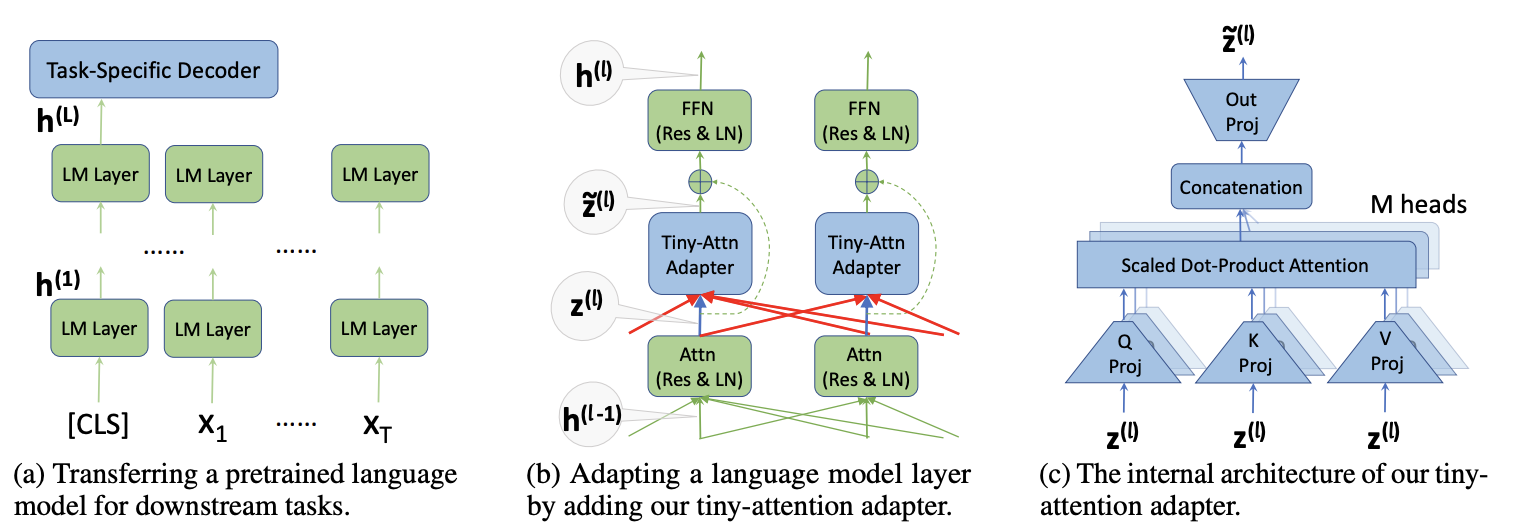
\includegraphics[width=0.8\textwidth]{chapter-2/tiny-attention.png}
    \caption{Arsitektur \textit{Tiny-Attention Adapter}}
    \label{fig:tiny-attention}
\end{figure}


Meskipun pendekatan ini terfokus pada efisiensi parameter, \textit{Tiny-Attention Adapter} tidak mengorbankan kinerja. Sebaliknya, berkat mekanisme "tiny-attention", teknik ini seringkali mampu mencapai kinerja yang sebanding atau bahkan melampaui metode adaptasi tradisional, meskipun hanya dengan sebagian kecil dari parameter tambahan.

Dengan demikian, \textit{Tiny-Attention Adapter} menawarkan pendekatan yang menjanjikan untuk mengadaptasi \textit{pre-trained model} dengan cara yang lebih efisien, tanpa mengorbankan kualitas atau kinerja.
\subsection{\textit{Prefix-Tuning}}

\textit{Prefix-Tuning} adalah teknik yang diperkenalkan untuk mengoptimalkan prompt kontinu dalam generasi teks. Berbeda dengan pendekatan tradisional yang melibatkan \textit{training} ulang seluruh model atau menambahkan parameter tambahan, \textit{Prefix-Tuning} fokus pada pengoptimalan sejumlah kecil parameter yang didefinisikan sebagai "prefix" dari sekuens input \parencite{prefix_tuning}. Dengan kata lain, alih-alih mengubah seluruh model, hanya \textit{prefix} dari input yang dioptimalkan untuk meningkatkan kinerja generasi.

\begin{figure}[ht]
    \centering
    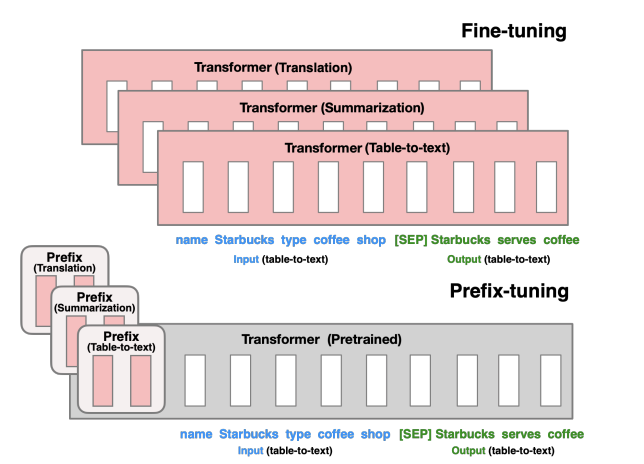
\includegraphics[width=0.8\textwidth]{chapter-2/prefix-tuning.png}
    \caption{Arsitektur \textit{Prefix-Tuning} \parencite{prefix_tuning}}
    \label{fig:prefix-tuning}
\end{figure}

Keuntungan utama dari pendekatan ini adalah efisiensi. Dengan mengoptimalkan hanya sebagian kecil dari parameter, \textit{Prefix-Tuning} dapat mencapai peningkatan kinerja dengan \textit{overhead} komputasi yang jauh lebih rendah dibandingkan dengan teknik \textit{fine-tuning} tradisional. Selain itu, dengan fokus pada \textit{prefix}, teknik ini memungkinkan adaptasi yang lebih spesifik terhadap tugas atau domain tertentu, memberikan fleksibilitas lebih dalam aplikasi praktis.

Teknik ini dapat digunakan untuk meningkatkan kinerja model generatif di berbagai tugas, termasuk penerjemahan mesin, peringkasan teks, dan lainnya. Hasil eksperimen menunjukkan bahwa \textit{Prefix-Tuning} mampu mencapai kinerja yang sebanding atau bahkan lebih baik dibandingkan dengan metode \textit{fine-tuning} tradisional, tetapi dengan biaya komputasi yang jauh lebih rendah.


\subsection{\textit{Unified View of Parameter-Efficient Transfer Learning}}

\textit{Unified Parameter Transfer Learning} merupakan strategi dalam \textit{transfer learning} yang berupaya menggabungkan berbagai teknik adaptasi ke dalam satu kerangka kerja terpadu \parencite{uvpl}. Tujuan utamanya adalah untuk memaksimalkan efisiensi dan efektivitas saat mengadaptasi \textit{pre-trained model} untuk tugas-tugas baru.

Dalam \textit{transfer learning}, ide utamanya adalah mengambil model yang telah dilatih pada satu tugas dan menyesuaikannya untuk tugas yang berbeda. Namun, ada banyak cara untuk melakukan adaptasi ini, dan setiap metode memiliki kelebihan dan kekurangannya sendiri. Beberapa teknik mungkin fokus pada penambahan lapisan adaptasi, sementara yang lain mungkin memprioritaskan modifikasi parameter tertentu dalam model.

Alih-alih memilih satu teknik adaptasi dan berkomitmen padanya, pendekatan ini menggabungkan berbagai teknik untuk menciptakan solusi adaptasi yang lebih komprehensif. Dengan demikian, model yang diadaptasi dengan metode ini dapat memanfaatkan kelebihan dari berbagai teknik adaptasi, sambil menghindari atau meminimalkan kekurangan masing-masing teknik.

Misalnya, satu teknik adaptasi mungkin sangat efektif untuk tugas klasifikasi tetapi kurang optimal untuk tugas generasi teks. Dengan pendekatan terpadu, model dapat memanfaatkan teknik adaptasi yang paling sesuai untuk setiap tugas, memungkinkan kinerja yang lebih baik dan adaptasi yang lebih cepat.

\begin{figure}[ht]
    \centering
    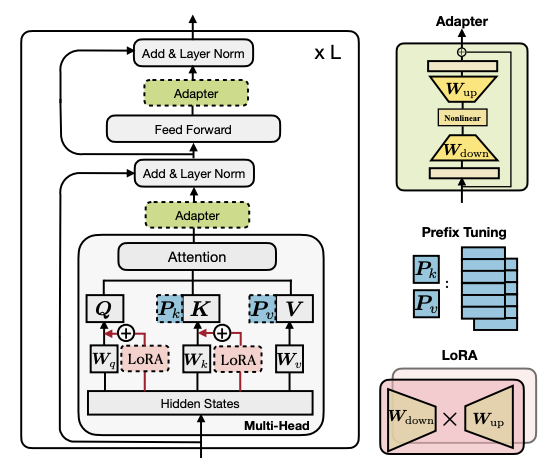
\includegraphics[width=0.8\textwidth]{chapter-2/uvpl.png}
    \caption{Arsitektur \textit{Unified View of Parameter-Efficient Transfer Learning} \parencite{uvpl}}
    \label{fig:uvpl}
\end{figure}

Selain itu, dengan menggabungkan berbagai teknik, \textit{Unified View of Parameter-Efficient Transfer Learning} juga memungkinkan peneliti untuk bereksperimen dan menemukan kombinasi teknik yang paling efektif untuk tugas atau dataset tertentu. Ini memberikan fleksibilitas tambahan dan memungkinkan adaptasi yang lebih disesuaikan dengan kebutuhan spesifik.


\section{\textit{NLP Task Benchmarking}}

Dalam pemrosesan bahasa alami (NLP), pentingnya evaluasi kinerja model pada berbagai tugas tidak dapat diremehkan. Evaluasi memberikan cara standar untuk membandingkan berbagai model dan teknik dalam konteks aplikasi nyata.

\subsection{\textit{General Language Understanding Evaluation} (GLUE)}

GLUE, yang merupakan singkatan dari \textit{General Language Understanding Evaluation}, adalah inisiatif yang dirancang untuk memajukan pemahaman bahasa alami melalui evaluasi yang konsisten dan komprehensif \parencite{glue}. Dengan latar belakang yang semakin meningkatnya kompleksitas dan variasi model NLP, muncul kebutuhan untuk memiliki metrik evaluasi yang standar dan konsisten. 

Salah satu ciri khas dari GLUE adalah kumpulan tugas evaluasinya yang beragam. Ini mencakup tugas-tugas seperti analisis sentimen, dengan tujuannya adalah untuk menentukan apakah teks tertentu memiliki konotasi positif, negatif, atau netral; jawaban pertanyaan, dengan model diberi pertanyaan dan harus memilih jawaban yang paling tepat dari kumpulan pilihan; dan entailment teks, dengan model harus menentukan apakah satu kalimat secara logis mengikuti kalimat lain.

Namun, bukan hanya variasi tugas yang membuat GLUE menjadi penting. GLUE juga menyediakan papan peringkat, yang memungkinkan peneliti untuk membandingkan kinerja model mereka dengan model-model lain dalam kondisi yang sama. Selain itu, GLUE juga memberikan kesempatan bagi peneliti untuk memahami kelemahan dan kekuatan model mereka. Dengan memiliki berbagai tugas evaluasi, peneliti dapat melihat kelemahan dari model yang berguna untuk mengembangkan model.
\subsection{IndoLEM}
% TODO: jelasin proses eksperimen saat ini, dan datasetnya juga 
IndoLEM muncul sebagai respons terhadap kebutuhan industri dan komunitas penelitian untuk memiliki \textit{benchmark} yang khusus dirancang untuk mengevaluasi model NLP dalam konteks bahasa Indonesia \parencite{indolem}. Meskipun ada banyak \textit{benchmark} NLP yang tersedia, seperti GLUE, kebanyakan dari mereka berfokus pada bahasa Inggris. Namun, dengan keragaman linguistik yang kaya, bahasa Indonesia memerlukan pendekatan khusus dalam evaluasi model NLP.

IndoLEM tidak hanya menyediakan kumpulan tugas evaluasi yang dirancang khusus untuk bahasa Indonesia, tetapi juga memastikan bahwa tugas-tugas tersebut mencerminkan nuansa dan tantangan unik yang diasosiasikan dengan bahasa ini. Salah satu aspek penting dari IndoLEM adalah dataset yang digunakannya. Mengingat pentingnya data dalam \textit{training} dan evaluasi model NLP, IndoLEM memastikan bahwa dataset yang digunakan berasal dari sumber-sumber lokal yang relevan. Ini memastikan bahwa model yang dievaluasi dengan IndoLEM benar-benar diuji dalam konteks yang sesuai dengan penggunaan sebenarnya dalam kehidupan nyata.
